\documentclass{article}
\usepackage{./em_tech,times}

\usepackage{amssymb, amsmath}
\usepackage{graphicx, subfigure}
\usepackage{hyperref}


\usepackage{color}

\newcommand{\argmax}{\operatornamewithlimits{argmax}}
\newcommand{\argmin}{\operatornamewithlimits{argmin}}


\title{Car Detection Using Depth Pano}


\author{
Andrew Taber \\
Earthmine Inc.\\
2390A 4th Street\\
Berkeley, CA 94703 \\
\texttt{andrew.taber@earthmine.com} \\
}

\newcommand{\fix}{\marginpar{FIX}}
\newcommand{\new}{\marginpar{NEW}}

\begin{document}

\maketitle

\begin{abstract}
earthmine's current implementation of license plate detection uses a height threshold to shrink the 
search space for a given panorama. This approach, while effectively shrinking the search space by at least 
half, does not incoporate any other depth data than the height. This article explores a new research path
attempting to use depth data to segment a panorama and increase both speed and accuracy of license plate
detection.
\end{abstract}

\section{Introduction}
Typically, implementations of license plate detection are in O($n^2 + m^2$), where n is the 
cardinality of the subset of the full image and m is the size of the feature convolution window. 
Therefore, it greatly benefits to heuristically narrow the search subset. We propose that using
depth discontinuity will provide such a heuristic. In particular, we consider height disparities
and use them to detect car faces, and so discard even more pixels from our sampling subset. 

\section{Algorithm Description}
After loading the depth and plano panoramas, and plane palette files, and finding the ground plane, we sample
the depth panorama, throwing away points that are further than 10 meters away from the camera, or are not between
.2 and 1 meters in height, and then writing their height values to an 2D array. After replacing each pixel in this 
array with its local standard deviation (essentially filtering out noise from actual height discontinuities), 
we segment the image in a three step process:

\begin{enumerate}
\item Use binary dilation to make data more dense (common problem in using depth data is sparseness of valid points)
\item Use binary closing to make data cluster together more
\item Label connected components
\end{enumerate}

Note that the structural elements for each of these steps is the same (a $3\times 3$ array filled with 1's). These 
functions are provided by scipy's ndimage.morphology module. 
\\

	Then, the labeled components are used to draw boxes around each component, both in the top-down view of the scene and in the panorama. 
Now, while we have achieved the original goal of segmenting the image for cars, we can further use the top-down data to
detect orientations of cars, and use these orientations to artificially rotate the RGB car image, thereby increasing accuracy since license plate detection has a much higher accuracy rate if the license plate is orthogonal to the camera.
\\

	Though this part of the algorithm is not complete, we present it's proposed implementation for completeness. At this point, we take the segmented top-down height map and for each component, applying the Hough transform to points within the component's bounding box. This gives a parametrization of line that goes through most points. This gives one line on which to project the RGB image, the other will be found orthogonal to this one. 

\section{Result}
The algorithm does very well in detecting cars with high accuracy and low false positive rate. 

\begin{figure}[htbp]
  \begin{center}
    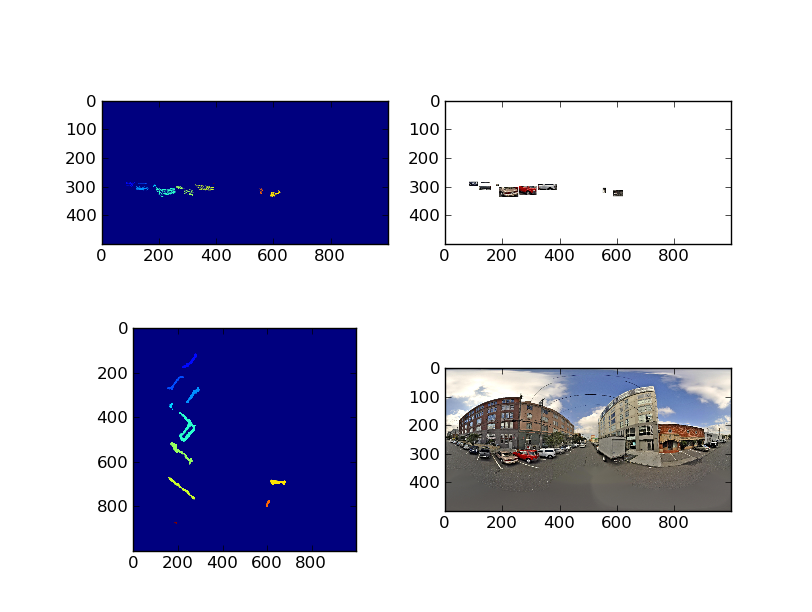
\includegraphics[height=9cm, width=12cm]{./object_detect.png}
  \end{center}
  \caption{Figure 1 (clockwise from top left): labeled points in pano space, segmented RGB subset, 2D height map (labeled) and full RGB pano}
\end{figure} 

However, the program itself takes at least 2 minutes to run to completion. This computational cost may be greatly reduced by porting this prototype code (written in Python) to C++, but it may still exceed the time taken by the brute force method. 

\section{Future Work}
The most fruitful future research path is finishing the part of the algorithm that takes the most likely line in each box and projects the RGB image onto the plane it represents. Presumably, this will make the algorithm much more accurate at detecting license plates, and might even be a novel enough solution to patent. 
 
\end{document}
